\section{Approach}
We followed a user-centered, iterative design process to develop SenseMap as a tool supporting browser-based online sensemaking. First, we identified current user behaviors in sensemaking using existing browser functionality. These behaviors led to the selection and subsequent development of a sensemaking model for user behaviors on the web. We conducted a series of design workshops to derive requirements from these user behaviors and model, then to design, build and test prototypes in an agile setting. Finally, the prototype was evaluated in a naturalistic work setting. \autoref{fig:sm-design-process} summarizes this process.

\begin{figure}[!htb]
	\centering
	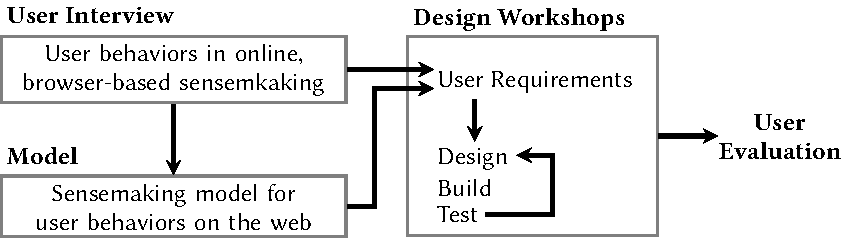
\includegraphics{design-process}
	\caption{Summary of the design process.}
	\label{fig:sm-design-process}
\end{figure}

\subsection{Design Research}
We conducted a semi-structured interview with nine participants to explore their behaviors in  conducting online sensemaking for their daily work activities. The interview happened during a normal working day to access the currently open, in-use browsers of participants, as a representative artifact of their practice. Therefore, the participant's browser became the scaffold for the conversation and provided the ongoing probes as the conversation unfolded. This method also ensured that participants described about what they actually did rather than talking about what they thought they did or should do.

We took video of each interview with the camera showing the interviewee's laptop screen and their hand gestures. We also made screen recordings of each laptop while the interview was taking place. \autoref{fig:sm-design-research} shows the combination of hand gesture and laptop screen of a participant. Each interview began with the participant showing their currently open browser windows. Browser choice was discussed and then the ongoing conversations were guided by five browser functions: searching, tabs, windows, bookmarks and history, with participants illustrating their behaviors using their in-use browsers. These behaviors are summarized as follows.

\begin{figure}
	\centering
	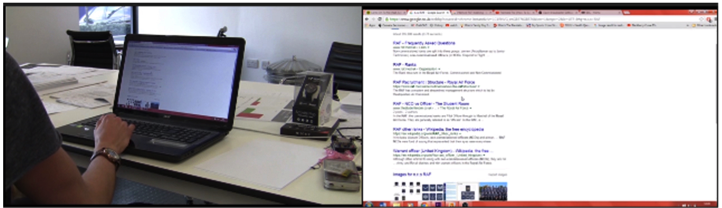
\includegraphics[width=\linewidth]{design-research}
	\caption{Interviewee's hand gesture and laptop screen.}
	\label{fig:sm-design-research}
\end{figure}

\paragraph{Starting Searches}
Opening a new tab preceded most searches. Users spoke about new tabs helping them to manage information, keep things separate and how they could go back to other pages that were relevant to their work activities and ongoing investigations.

\paragraph{Tabs}
Eight of the nine participants had a number of tabs open and categorized them as either: collections of tabs relating to current investigations or single points of access to commonly accessed services, e.g. social feeds, email etc. In further probing about the tab collections a number of shared behaviors emerged.

\begin{enumerate}
	\item Opening a new tab if ``significant'' information is found enabling the page to stay live in the browser.
	\item Opening Google search result links in a series of new tabs from one search page. Subsequent tabs were reviewed and then kept or closed based on their significance.
	\item Reordering tabs to develop a narrative. In all cases the narrative was described as flowing from left to right. The narrative was used by the participants to make sense of the information found, to develop more refined search strategies and terms where information was lacking, and to communicate their findings to others.
	\item All participants expressed anxiety about losing tabs when they were inadvertently closed or lost due to a system error and they all described the same recovery procedure using the recently closed tabs section of the History menu.
	\item The number of tabs in browser windows varied greatly across the participants. One participant diligently closed all tabs at the end of each ``work episode'' although sometimes they kept them open in a non-active window when at home and used a new window for private web browsing. Most described groups of seven to eight tabs that were currently in use for active projects. One user had over fifty tabs open in their main browser and twenty in their second browser, but they gave the same explanation for their presence, use and organization.
\end{enumerate}

\paragraph{Windows}
Only one user described the use of more than one window in the web browser. Similarly to Behavior 5, this enabled him to keep work-related tabs separate from private browsing.

\paragraph{Bookmarks}
There was considerable variance in the use of browser bookmarks although most had moved away from using them and relied instead upon tabs to keep relevant information live and accessible. Two participants had no bookmarks at all.  One participant saved some bookmarks, but these were not organized into groups, categories or folders. One participant described a behavior where they bookmark the contents of tabs at the conclusion of a project and organize these into named folders. However, they rarely revisited these bookmarks to use them to access information again, instead preferring ``Pinterest'' or relying on Google to find it again from a search term.

\paragraph{History}
None of the participants made use of the history menu to revisit pages or to make sense of recorded information. However, all of them used it to reestablish a tab if it had been inadvertently closed.

\subsection{Sensemaking Model}
We considered the relevance of extant sensemaking models to the elicited behaviors, principally Pirolli and Card's model and Data--frame model (Literature Review chapter, \autoref{sub:lr-sensemaking}). The iterative process of sensemaking described by Pirolli and Card effectively encapsulates the observed tab behaviors:

\begin{itemize}
	\item The \emph{foraging loop}: behaviors 1 and 2
	\item The \emph{sensemaking loop}: behavior 3
	\item Behaviors 4 and 5 indicate possible tool features rather than a step described in Pirolli-Card model.
\end{itemize}

The synthesis of our observed behaviors with the Pirolli and Card's model indicates a browser-based sensemaking process, during which information sources are held in a \textit{collection} of browser tabs (foraging loop), with each tab containing the provenance for the source. An ongoing \textit{curation} process (sensemaking loop) takes place where tabs are ordered into categories and a narrative sequence unfolds within such categorized groups. These groups and relationships represent the underlying schema. The results of the curation are then used to guide further more refined searches and, on completion, as a support to \textit{communicate} the findings to others. \autoref{fig:sm-refined-sensemaking-model} illustrates our refined model.

\begin{figure}[!htb]
	\centering
	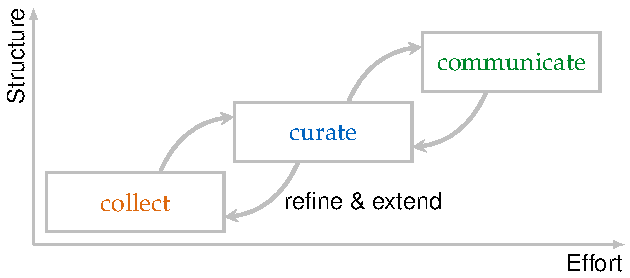
\includegraphics{refined-sensemaking-model}
	\caption{Our refined sensemaking model for user behaviors on the web.}
	\label{fig:sm-refined-sensemaking-model}
\end{figure}

\subsection{Design Workshops}
We organized a series of iterative design workshops to derive and satisfy requirements with an overall aim to support and augment current browser-based online sensemaking activities. In the first workshop, an initial design was proposed, detailing visual representation and user interaction. A prototype was built based upon this proposal, and subsequent workshops sought to develop this tool through the ongoing interplay between design, build and test in an agile setting.

We will describe the requirements next and present the interface design in \autoref{sec:sm-design}. Some of these requirements link directly to observed behaviors, some are inferred from our sensemaking model, and some are produced during creative design processes set within the constraints of the technology platform chosen.

\subsubsection{Collection Requirements}

\begin{enumerate}
	\item \textbf{Rich provenance}: enrich and make the provenance of information sources more visible to users. Currently, the provenance of tabs is only accessible when they are active and then only by a list of page titles (in Chrome, press and hold the browser's back button), which requires users to build their own schema that is external to the browser.
	\item \textbf{Easy revisitation}: provide quick and easy mean to revisit the information sources needed. Our interviews show that users often revisit their important tabs (Behaviors 1 and 2), but rarely use bookmarks and history. During a session, they rely on the tab titles, their memories or trial-and-error. However, tab titles are represented by a favorite icon and a truncated page title, which is a poor abstraction from the original source. This abstraction becomes poorer as more tabs are opened, making revisitation difficult when tab collections are large.
	\item \textbf{Location awareness}: provide an overview of the sensemaking process to address the disorientation problem~\cite{Conklin1987}, enabling users to know what they have done so far, where they are in the context of the overall tasks, and potentially guide the next step.
	\item \textbf{Preparation for curation}: provide highlight and annotation support for users, which can facilitate more elaborate thinking~\cite{Sedig2013}, and can serve as a step to assess the relevance of the information sources. The information representation should have different levels of richness depending on the assessed relevance.
	\item \textbf{Interruption \& Separation}: enable task switching without compromising the collection process; for instance, checking email or social feeds should not get recorded as part of the sensemaking process (Behavior 5).

	\setcounter{listnum}{\theenumi}
\end{enumerate}

\subsubsection{Curation Requirements}

\begin{enumerate}
	\setcounter{enumi}{\thelistnum}
	\item \textbf{Rich representation}: provide a rich abstraction of the information source allowing the user to quickly recognize it~\cite{Tauscher1997}. This also relates to the ``Easy revisitation'' and ``Location awareness'' requirements for Collection.
	\item \textbf{Spatial organization}: enable users to freely arrange information sources in both $x$ and $y$ dimensions to address the limit of a one-dimensional sequence of tabs being used to visualize multiple narrative threads (Behavior 3). Spatial organization plays an important role in sensemaking~\cite{Sedig2013}, especially with a large space~\cite{Andrews2010}.
	\item \textbf{Linking/unlinking}: enable further curation of these sources by establishing links, which is impossible with existing browsers. Linking and unlinking are also known to help users to produce more critical thinking~\cite{Sedig2013}.
	\item \textbf{Formal reasoning}: enable users to apply formal argumentation methods such as Toulmin's argument~\cite{Toulmin2003} or Wigmore's chart~\cite{Goodwin2000}. We think that they may be helpful when solving complex sensemaking tasks analytically.
	\item \textbf{Collection -- Curation}: enable users to see connections between the curated and collected sources, and to use these to inform further searches. This is to support the ``refine and extend'' direction in our sensemaking model (\autoref{fig:sm-refined-sensemaking-model}).

	\setcounter{listnum}{\theenumi}
\end{enumerate}

\subsubsection{Communication Requirements}

\begin{enumerate}
	\setcounter{enumi}{\thelistnum}
	\item \textbf{Complete picture}: provide a complete picture of the curated sources and the relationships that a user ascribes to them via their curation activity. Currently, it is impossible to see an overall picture of the curated sources and their categorization from the sequence of tabs.
	\item \textbf{Auditability}: enable users to refer to raw data as evidence supporting their reasoning, which is considered as an important characteristics in analytic presentation~\cite{Chinchor2009}.
	\item \textbf{Varied audience}: enable users to customize the curated set of information to suit various needs and backgrounds of the audience. This is also another important characteristic in analytic presentation~\cite{Chinchor2009}.
	\item \textbf{Sharing}: enable users to share both raw and curated sets of information with others. This is a first step toward a collaborative environment for online sensemaking.
\end{enumerate}